%!TEX root = ../thesis.tex
%Adding the above line, with the name of your base .tex file (in this case "thesis.tex") will allow you to compile the whole thesis even when working inside one of the chapter tex files

\chapter{Targets, Instrumentation, and Observations} \label{chap:3}

\section{Betelgeuse}\label{sec:3.1}
decin proposal, paper intro, CO

\begin{table}
\begin{center}
\caption[Physical Properties of $\alpha$ Ori.]
{Physical Properties of $\alpha$ Ori.}
\begin{tabular}{lcc}
\hline
\hline
\rule{0pt}{2.5ex}Property & $\alpha$ Ori & Reference \\
\hline
\rule{0pt}{2.5ex}HD Number & 124897 & \\
Spectral Type & K2 III &\\ 
ra (ICRS: ep=J2000)&14$^{\rm{h}}$15$^{\rm{m}}$39.672$^{\rm{s}}$&\\
dec (ICRS: ep=J2000) & +19 10 56.673 & \\
pm-ra (mas yr$^{-1}$)& $-1093.39 \pm 0.44$ & \\
pm-dec (mas yr$^{-1}$)& $-2000.06 \pm 0.39$ & \\
$\pi$ (mas)& $88.83\pm 0.54$ &\\
Distance (pc)& 11.3$\pm$0.1 & \\
$M$ ($M_{\odot}$) & 0.8$\pm$0.2 & \\
$\theta _{\rm{UD}}$ (mas)& 21.0$\pm$0.2 & \\
$\theta _{\rm{LD}}$ (mas)& 21.0$\pm$0.2 & \\
L ($L_{\odot}$)& &  \\
$R$ ($R_{\odot}$)& 25.4$\pm$0.3 & \\
Log $g$ & &  \\
$T_{\rm{eff}}$ (K) & 4294$\pm$30 & \\
$v_{\rm{rad}}$ (km s$^{-1}$) & $+5.19 \pm 0.04$ & \\
$v_{\rm{esc}}$ (km s$^{-1}$) &110 & \\
$v_{\rm{\infty}}$ (km s$^{-1}$)& $\sim$40 & \\
$T_{\rm{wind}}$ (K)& $\sim$10,000 & \\
$\dot{M}$ ($M_{\odot}$ yr$^{-1}$)& \\
$H$ ($H_{\odot}$)& & \\
 Fe/H& -0.5$\pm$0.2 &\\
\hline
\rule{0pt}{2.5ex}
\end{tabular}
\label{tab:3.1}
\end{center}
\end{table}

\section{CARMA}\label{sec:3.2}

%The VLA's resolution is generally diffraction-limited, and thus is set by the array configuration and frequency of observation. It is important to be aware that a synthesis array is "blind" to structures on angular scales both smaller and larger than the range of fringe spacings given by the antenna distribution. For the former limitation, the VLA acts like any single antenna - structures smaller than the diffraction limit (θ ∼ λ/D) are not seen -- the resulting image will be smoothed to the resolution of the array. The latter limitation is unique to interferometers; it means that structures on angular scales significantly larger than the fringe spacing formed by the shortest baseline are not measured. No subsequent processing can fully recover this missing information, which can only be obtained by observing in a smaller array configuration, by using the mosaicing method, or by utilizing data from an instrument (such as a large single antenna or an array comprising smaller antennas) which provides this information.


\section{CARMA Observations of Betelgeuse}\label{sec:3.3}
3 configurations, max and min resolutions, variability of phase cals, flux cals
\begin{landscape}
\begin{table}
\begin{center}
\caption[CARMA Observations of $\alpha$ Ori.]
{CARMA Observations of $\alpha$ Ori between June 2007 and November 2009.}
\begin{tabular}{lccccc}
\hline
\hline
\rule{0pt}{2.5ex}Date & Configuration & Time on Source & Flux		& Phase 	& Image Cube \\
	 & 				 &  (hr)		  & Calibrator	& Calibrator& Dynamic Range \\
\hline
\rule{0pt}{2.5ex}2007 Jun 18 	& D & 0.9 & 0530+135	& 0530+135, 0532+075 	&  22.8 \\
2007 Jun 21 	& D & 3.0 & 0530+135	& 0530+135, 0532+075 	&  22.7 \\
2007 Jun 24 	& D & 2.1 & 0530+135	& 0530+135, 0532+075 	&  26.1 \\
2007 Jun 25 	& D & 2.4 & 0530+135	& 0530+135, 0532+075 	&  30.2 \\
2009 Jul 07	& E & 3.2 & 3C120 		& 3C120, 0532+075	& 30.1 \\
2009 Nov 05	& C & 1.2 & 3C120 		& 3C120, 0532+075 	& 17.3 \\
2009 Nov 09 	& C & 3.0 & 3C120 		& 3C120, 0532+075 	& 27.2 \\
2009 Nov 15	& C & 1.0 & 3C120 		& 3C120, 0532+075 	& 17.8 \\
2009 Nov 16	& C & 3.2 & 3C120 		& 3C120, 0532+075 	& 32.0  \\
All		& C & 8.4	&  $\dots$	& 	$\dots$	& 43.8 \\
All 		& D & 8.4 &  $\dots$	&  	$\dots$	& 31.9 \\
All 		& Multi-configuration & 20.0 & $\dots$& $\dots$ 	& 52.3 \\
\hline
%\tablenotetext{a}{Central frequency of selected bandpass.}
%\tablenotetext{b}{Number of available antennae remaining after flagging.}
\end{tabular}
\label{tab:1}
\end{center}
\end{table}
\end{landscape}

\section{Arcturus and Aldebaran}\label{sec:3.4}
wood paper, paper into, ken proposal re arcturus
\begin{table}
\begin{center}
\caption[Physical Properties of $\alpha$ Boo and $\alpha$ Tau.]
{Physical Properties of $\alpha$ Boo and $\alpha$ Tau.}
\begin{tabular}{lccc}
\hline
\hline
\rule{0pt}{2.5ex}Property & $\alpha$ Boo & $\alpha$ Tau & Reference\\
\hline
\rule{0pt}{2.5ex}HD Number & 124897 & 29139 & $\ldots$\\
Spectral Type & K2 III & K5 III& 1, 2\\ 
ra (ICRS: ep=J2000)&14$^{\rm{h}}$15$^{\rm{m}}$39.672$^{\rm{s}}$&04$^{\rm{h}}$35$^{\rm{m}}$55.239$^{\rm{s}}$&3\\
dec (ICRS: ep=J2000) & +19 10 56.673 & +16 30 33.489 & 3 \\
pm-ra (mas yr$^{-1}$)& $-1093.39 \pm 0.44$ & $63.45\pm 0.84$  & 3 \\
pm-dec (mas yr$^{-1}$)& $-2000.06 \pm 0.39$ & $-188.94\pm 0.65$ & 3 \\
$\pi$ (mas)& $88.83\pm 0.54$ & $48.94\pm 0.77$& 3\\
Distance (pc)& 11.3$\pm$0.1 & 20.4$\pm$0.3& 3\\
$M$ ($M_{\odot}$) & 0.8$\pm$0.2 & 1.3$\pm$0.3& 6, 4 \\
$\theta _{\rm{UD}}$ (mas)& 21.0$\pm$0.2 & 20.2$\pm$0.3& 5 \\
$\theta _{\rm{LD}}$ (mas)& 21.0$\pm$0.2 & 20.2$\pm$0.3& 5 \\
L ($L_{\odot}$)& & & \\
$R$ ($R_{\odot}$)& 25.4$\pm$0.3 & 44.4$\pm$1.0 & $\ldots$ \\
Log $g$ & & & \\
$T_{\rm{eff}}$ (K) & 4294$\pm$30 & 3970$\pm$49& 5 \\
$v_{\rm{rad}}$ (km s$^{-1}$) & $+5.19 \pm 0.04$ & $+54.11\pm 0.04$ & 9\\
$v_{\rm{esc}}$ (km s$^{-1}$) &110 & 106& $\ldots$\\
$v_{\rm{\infty}}$ (km s$^{-1}$)& $\sim$40 & $\sim$30& 7, 8\\
$T_{\rm{wind}}$ (K)& $\sim$10,000 & $<$10,000 & 7, 8\\
$\dot{M}$ ($M_{\odot}$ yr$^{-1}$)& $2\times 10^{-10}$& $1.6\times 10^{-11}$& 7, 8\\
$H$ ($H_{\odot}$)& & & $\ldots$\\
Fe/H& -0.5$\pm$0.2 & 0.00$\pm$0.2 & 10\\
\hline
\end{tabular}
\label{tab:1}
\begin{minipage}{13.0cm}
References.-(1);(2)\cite{gray_2006}; (3)\cite{van_leeuwen_2007}; (5)\cite{di_benedetto_1993};
(6)\cite{kallinger_2010}; (7)\cite{drake_1985}; (8)\cite{robinson_1998}
(9)\cite{massarotti_2008}; (10)\cite{decin_2003}
\end{minipage}
\end{center}
\end{table}

\section{The Karl G. Jansky Very Large Array}\label{sec:3.5}
The Karl G. Jansky Very Large Array (VLA) is an aperture synthesis radio telescope located on the Plains of San Agustin, New Mexico, USA and is capable of producing radio images with a resolution comparable to that of optical telescopes. It is the product of a program to modernize the electronics of the `old' VLA which had been in operation since the late 1970's. One of the main upgrades to the VLA is the addition of the Wideband Interferometric Digital Architecture (WIDAR) correlator which allows the digital correlation of very wideband signals. WIDAR digitally filters and splits the data into sub-bands which are then separately cross-correlated and integrated before being stitched together again to yield the final wideband spectrum. The new WIDAR correlator and its superior bandwidth capability provides the VLA with greater sensitivity, allowing the detection of lower flux density sources than was previously possible with the `old' VLA. A comparison of the performance parameters of the VLA with those of the `old' VLA is shown in Table \ref{tab:3.1}. The three major new observational abilities of the VLA are:
\begin{enumerate}
\item Complete frequency coverage between 1 and 50 GHz.
\item An increase in continuum sensitivity by an order of magnitude at some frequencies, by increasing the bandwidth to 8 GHz per polarization.
\item Process the large bandwidth with a minimum of 16,384 spectral channels per baseline.
\end{enumerate}

\begin{table}
\begin{center}
\caption[Improved Performance Parameters of the VLA.]
{Improved Performance Parameters of the VLA.}
\begin{tabular}{lccc}
\hline
\hline
\rule{0pt}{2.5ex}Parameter & `old' VLA & VLA & Improvement Factor \\
\hline
\rule{0pt}{2.5ex}Continuum sensitivity (1$\sigma$, 9 hr) & 10 $\mu$Jy & 1 $\mu$Jy& 10\\
Bandwidth per polarization & 0.1 GHz & 8 GHz & 80\\ 
Coarsest frequency resolution & 50 MHz & 2 MHz & 25\\ 
Finest frequency resolution & 381 Hz & 0.12 Hz & 3180\\ 
Channels at max. bandwidth & 16 & 16,384 & 1024\\ 
Maximum number of channels & 512 & 4,194,304 & 8192\\ 
\hline
\end{tabular}
\label{tab:3.1}
\end{center}
\end{table}

Apart from the addition of more feeds at the center of the reflector, the structural design of the VLA has not changed during its recent upgrade. As before it consists of 27 fully steerable alt-azimuth antennas arranged along the arms of an upside-down `Y' as shown in Figure \ref{fig2.9}.  The array is reconfigurable and can vary its resolution by over a factor of $\sim 50$ through movement of its component antennas along twin railroad tracks. Four standard configurations of antennas along the arms of the array are possible whose scales vary by the ratios 1 : 3.28 : 10.8 : 35.5 from smallest to largest. These are called D, C, B, and A configurations, with A having the longest baselines ($\sim 36$ km) giving the best angular resolution, but lacking short baselines needed for imaging extended structure. In each configuration, the distance of each antenna from the center of the `Y' is equal to $m^{\rm{ln}2}$ where $m$ is the antenna location number, counting outwards from the center of each arm. With this design, the $m$'th station in any configuration coincides with the 2$m$'th station in the next smaller configuration. This means that only 72 stations are needed to handle all four configurations. Additionally, there are 3 `hybrid' configurations called DnC, CnB, and BnA, which are well suited for sources with low declinations. In these configurations, the North arm antennas are deployed in the next larger configuration than the SE and SW arm antennas resulting in a more circular dirty beam for these sources.

Each antenna is 25 m in diameter giving the array a total collecting area equivalent to a single dish of 130 m in diameter. Each antenna has an off-axis Cassegrain design with a rotatable sub-reflector at the prime focus of the main reflector supported by four feed legs. All feeds are located on a feed ring at the Cassegrain focus and the observing feed is changed by rotating the asymmetric sub-reflector about the main reflector axis so that the secondary focal point moves to the desired feed. The standard observing mode for all feeds is circular polarization. RF signals from each feed  are sent via a waveguide to the antenna vortex room located directly underneath the main reflector where they are feed into low noise front ends. The vortex room is temperature controlled and also contains cryogenic cooling systems for the front end, portions of the LO, and IF equipment. IF signals from each antenna are sent by cable to a shielded room where the sampler and delay and multiplier racks are located. Once the signals have been cross-correlated they are time averaged into visibility measurements.

\begin{figure}[hbt!]
\centering 
          \includegraphics[trim=0pt 220pt 0pt 220pt,clip,width=\textwidth]{/home/eamon/thesis/thesis_template/3/vla_antenna.ps}
\caption[x]{x}
\label{fig3.1}
\end{figure}

\begin{table}
\begin{center}
\caption[Frequency coverage, primary beam, and angular resolution of the VLA.]
{Frequency coverage, primary beam, and angular resolution of the VLA.}
\begin{tabular}{lcccccccc}
\hline
\hline
\rule{0pt}{2.5ex} &  L& S&C&X&Ku&K&Ka&Q\\
\hline
\rule{0pt}{2.5ex}$\nu$ (GHz)& 1.5& 3.0&6.0&10&15&22&33&45\\
$\lambda$ (cm)& 20& 13&6.0&3.0&2.0&1.3&1.0&0.7\\
$\nu$ Range (GHz)& 1-2& 2-4&4-8&8-12&12-18&18-26.5&26.5-40&40-50\\
FOV: $\theta_{\rm{HPBW}} ^{\rm{PB}}$ ($'$)& 30& 15&7.5 &4.5 &3.0&2.0&1.4&1.0\\
A config: $\theta_{\rm{HPBW}}^{\rm{SB}}$ ($\arcsec$)&  1.3& 0.65&0.33&0.20&0.13&0.089&0.059&0.043\\
B config: $\theta_{\rm{HPBW}}^{\rm{SB}}$ ($\arcsec$)&  4.3& 2.1&1.0&0.6&0.42&0.28&0.19&0.14\\
C config: $\theta_{\rm{HPBW}}^{\rm{SB}}$ ($\arcsec$)&  14& 7.0&3.5&2.1&1.4&0.95&0.63&0.47\\
D config: $\theta_{\rm{HPBW}}^{\rm{SB}}$ ($\arcsec$)&  46& 23&12&7.2&4.6&3.1&2.1&1.5\\
\hline
\end{tabular}
\label{tab:3.1}
\end{center}
\end{table}
All VLA antennas are outfitted with eight receivers providing continuous frequency coverage between 1 and 50 GHz. As shown in Table x, the frequency ranges of 1-2 GHz, 2-4 GHz, 4-8 GHz, 8-12 GHz, 12-18 GHz, 18-26.5 GHz, 26.5-40 GHz, and 40-50 GHz are commonly referred to as L, S, C, X, Ku, K, Ka, and Q bands, respectively. Additionally, the VLA is currently being outfitted with even lower frequency receivers, P-band (230-470 MHz) and 4-band (54-86 MHz). The VLA's angular resolution is set by the maximum baseline $B_{\rm{max}}$ and frequency of observation. This means that structures smaller than the diffraction limit ($\theta_{\rm{HPBW}}^{\rm{SB}} \sim \lambda/B_{\rm{max}}$) will be smoothed to the resolution of the array. Table x summarizes the maximum resolution for each of the four main configurations at each wavelength. The resolution is defined here as the HPBW of the synthesized beam, using uniform weighting, over a full 12 hour synthesis observation of a source which passes near the zenith. For completeness, we also give the field of view (FOV) at each observing frequency in Table x, defined as the HPBW  of the primary beam, which for the VLA antennas can be approximated using the formula: $\theta_{\rm{HPBW}} ^{\rm{PB}} (')= 45/\nu _{\rm{GHz}}$. 

\section{VLA Observations of Arcturus and Aldebaran}\label{sec:3.6}
The Open Shared Risk Observing (OSRO) program at the VLA existed during its commissioning phase to provide observers with early access to a number of VLA correlator capabilities and observing modes. This represented a considerable improvement over the capabilities of the old VLA correlator as observes were provided with increased bandwidth capability at existing VLA bands, increased spectral resolution capabilities, and access to new spectral bands. In September 2010 our proposal (PI: G. M. Harper, Program ID: 10C-105) to observe two archetypical red giants at multiple frequencies was allocated the requested 15.5 hours of observing time with the VLA as part of NRAO's OSRO Science Program 2010C. A number of observing scripts called scheduling blocks (SBs) were prepared during December 2010 and their duration were kept to $\leq 2.5$ hours to increase their likelihood of been scheduled. The VLA now uses dynamic scheduling for deciding which SBs are executed at any time. It takes into account many factors like the scheduling priority assigned by the time allocation committee, weather constraints, and SB duration. Dynamic scheduling means that the observer does not know when their observations will occur but in general, the chances of observations being scheduled are increased if the duration of the SB is kept small.

\begin{landscape}
\begin{table}
\begin{center}
\caption[VLA Observations of $\alpha$ Boo and $\alpha$ Tau.]
{VLA Observations of $\alpha$ Boo and $\alpha$ Tau obtained in February 2011 and July 2012.}
\begin{tabular}{lccccccccc}
\hline
\hline
\rule{0pt}{2.5ex}Star & Date & Band & $\nu$	& $\lambda$& Time on& Restoring Beam			& Bandwidth & Number of&Phase\\
	 & 		&  & (GHz)		& (cm)		& Star (hr)		  & ($\arcsec \times \arcsec$)& (GHz)		& Antennas&Calibrator\\
\hline
\rule{0pt}{2.5ex} $\alpha$ Boo 	& 2011 Feb 22 & Q	& 43.3 & 0.7		& 0.3 	&0.19 $\times$ 0.15& 0.256	&22& J1357+1919  \\
				& 2011 Feb 22 & Ka	& 33.6 & 0.9		& 0.2 	&0.25 $\times$ 0.20& 0.256 	&23&J1357+1919  \\
				& 2011 Feb 22 & K	& 22.5 & 1.3		& 0.4	&0.35 $\times$ 0.28& 0.256 	&24&J1357+1919  \\
				& 2011 Feb 11 & X	& 8.5  & 3.5		& 0.3 	&1.14 $\times$ 0.70& 0.256 	&18&J1415+1320  \\
				& 2011 Feb 11 & C	& 5.0  & 6.0 		& 0.5	&2.02 $\times$ 1.30& 0.256 	&21& J1415+1320 \\
				& 2011 Feb 13 & S	& 3.1  & 9.5 		& 1.8 	&2.57 $\times$ 2.08& 0.256 	&12& J1415+1320 \\
				& 2012 Jul 19 & S	& 3.0  & 10.0 		& 0.7 	&2.82 $\times$ 2.30& 2.0		&23& J1415+1320 \\
				& 2012 Jul 20 & L	& 1.5  & 20.0		& 1.6 	&4.46 $\times$ 3.94& 1.0		&23& J1415+1320 \\
\hline
\rule{0pt}{2.5ex}  $\alpha$ Tau	& 2011 Feb 11 & Q	& 43.3 & 0.7 		& 0.3 	&0.18 $\times$ 0.16& 0.256 	&22&  J0431+1731\\
				& 2011 Feb 11 & Ka	& 33.6 & 0.9 		& 0.2 	&0.22 $\times$ 0.20& 0.256 	&19&  J0449+1121\\
				& 2011 Feb 11 & K	& 22.5 & 1.3 		& 0.4 	&0.35 $\times$ 0.31& 0.256 	&21&  J0449+1121\\
				& 2011 Feb 13 & X	&  8.5 & 3.5 		& 0.5	&0.85 $\times$ 0.78& 0.256 	&25&  J0449+1121\\
				& 2011 Feb 13 & C	&  5.0 & 6.0 		& 1.2	&1.48 $\times$ 1.32& 0.256 	&21&  J0449+1121\\
				& 2011 Feb 12 & S	&  3.1 & 9.5 		& 1.8 	&2.74 $\times$ 2.02& 0.256 	&11&  J0431+2037\\ 
\hline
%\tablenotetext{a}{Central frequency of selected bandpass.}
%\tablenotetext{b}{Number of available antennae remaining after flagging.}
\end{tabular}
\label{tab:1}
\end{center}
\end{table}
\end{landscape}

Our main set of observations took place in February 2011 while the VLA was in B-configuration. All observations were taken in continuum mode and the correlator was set up with two 128 MHz sub-bands centered on the frequencies listed in Table x. Each sub-band had sixty-four channels of width 2 MHz and four polarization products (RR, LL, RL, LR). We obtained all our requested observations of $\alpha$ Tau in just two days between the 11$^{\rm{th}}$ and 13$^{\rm{th}}$ of February 2011 which consisted of Q, Ka, K, X, C, and S band observations of the star. We did not request L band (i.e. 1.5 GHz) observations of $\alpha$ Tau as it was believed that the star would be too faint to be observable at this frequency. There was also insufficient Ku band receivers available at the time to carry out observations at 15 GHz. We obtained Q, Ka, K, X, C, and S band observations of $\alpha$ Boo in ten days between the 11$^{\rm{th}}$ and 22$^{\rm{nd}}$ of February 2011. We also had prepared a 2.5 hour SB for $\alpha$ Boo at L-band but this SB was never executed. 

For this reason we applied for (and were awarded) 3 additional hours of directors discretionary time (DDT) in early 2012 (PI: E. O'Gorman, Program ID: 12A-472) to observe $\alpha$ Boo at S and L band. We decided to include a short observation at S band even though we already had an observation at this band to make sure that the stars flux density had not significantly changed over that period and so any possible L band detection could be included in the analysis of the main set of data from the previous year. Our DDT observations took place in July 2012 when the VLA was again in B-configuration and some of the details are again given in Table x. The capabilities of the VLA had increased drastically in the $\sim 1.5$ years since the main set of observations and we now could utilize the full 1 and 2 GHz of bandwidth at L and S band, respectively. The 1-2 GHz and 2-4 GHz frequency ranges were both divided into 16 sub-bands, each with sixty-four channels. The channel width was 2 and 1 MHz for S and L-band, respectively, and each sub-band had four polarization products (RR, LL, RL, LR).

\begin{figure}[hbt!]
\centering 
\mbox{
          \includegraphics[trim=35pt 0pt 50pt 0pt,clip,width=7.0cm,height=7.5cm,angle=270]{/home/eamon/thesis/thesis_template/3/phase_center1.ps}
          \includegraphics[trim=35pt 100pt 50pt 0pt,clip,width=7.0cm,height=7.5cm,angle=270]{/home/eamon/thesis/thesis_template/3/phase_center2.ps}
          }
\caption[x]{x}
\label{}
\end{figure}

\begin{figure}[hbt!]
\centering 
\mbox{
          \includegraphics[trim=35pt 0pt 50pt 0pt,clip,width=7.0cm,height=7.5cm,angle=270]{/home/eamon/thesis/thesis_template/3/atau_cx.ps}
          \includegraphics[trim=35pt 100pt 50pt 0pt,clip,width=7.0cm,height=7.5cm,angle=270]{/home/eamon/thesis/thesis_template/3/atau_kkaq.ps}
          }
\caption[x]{x}
\label{}
\end{figure}